\frontmatter
\pagestyle{empty}

% cover
\tikz[remember picture,overlay]
    \node[opacity=1.0,inner sep=0pt] at (current page.center){
        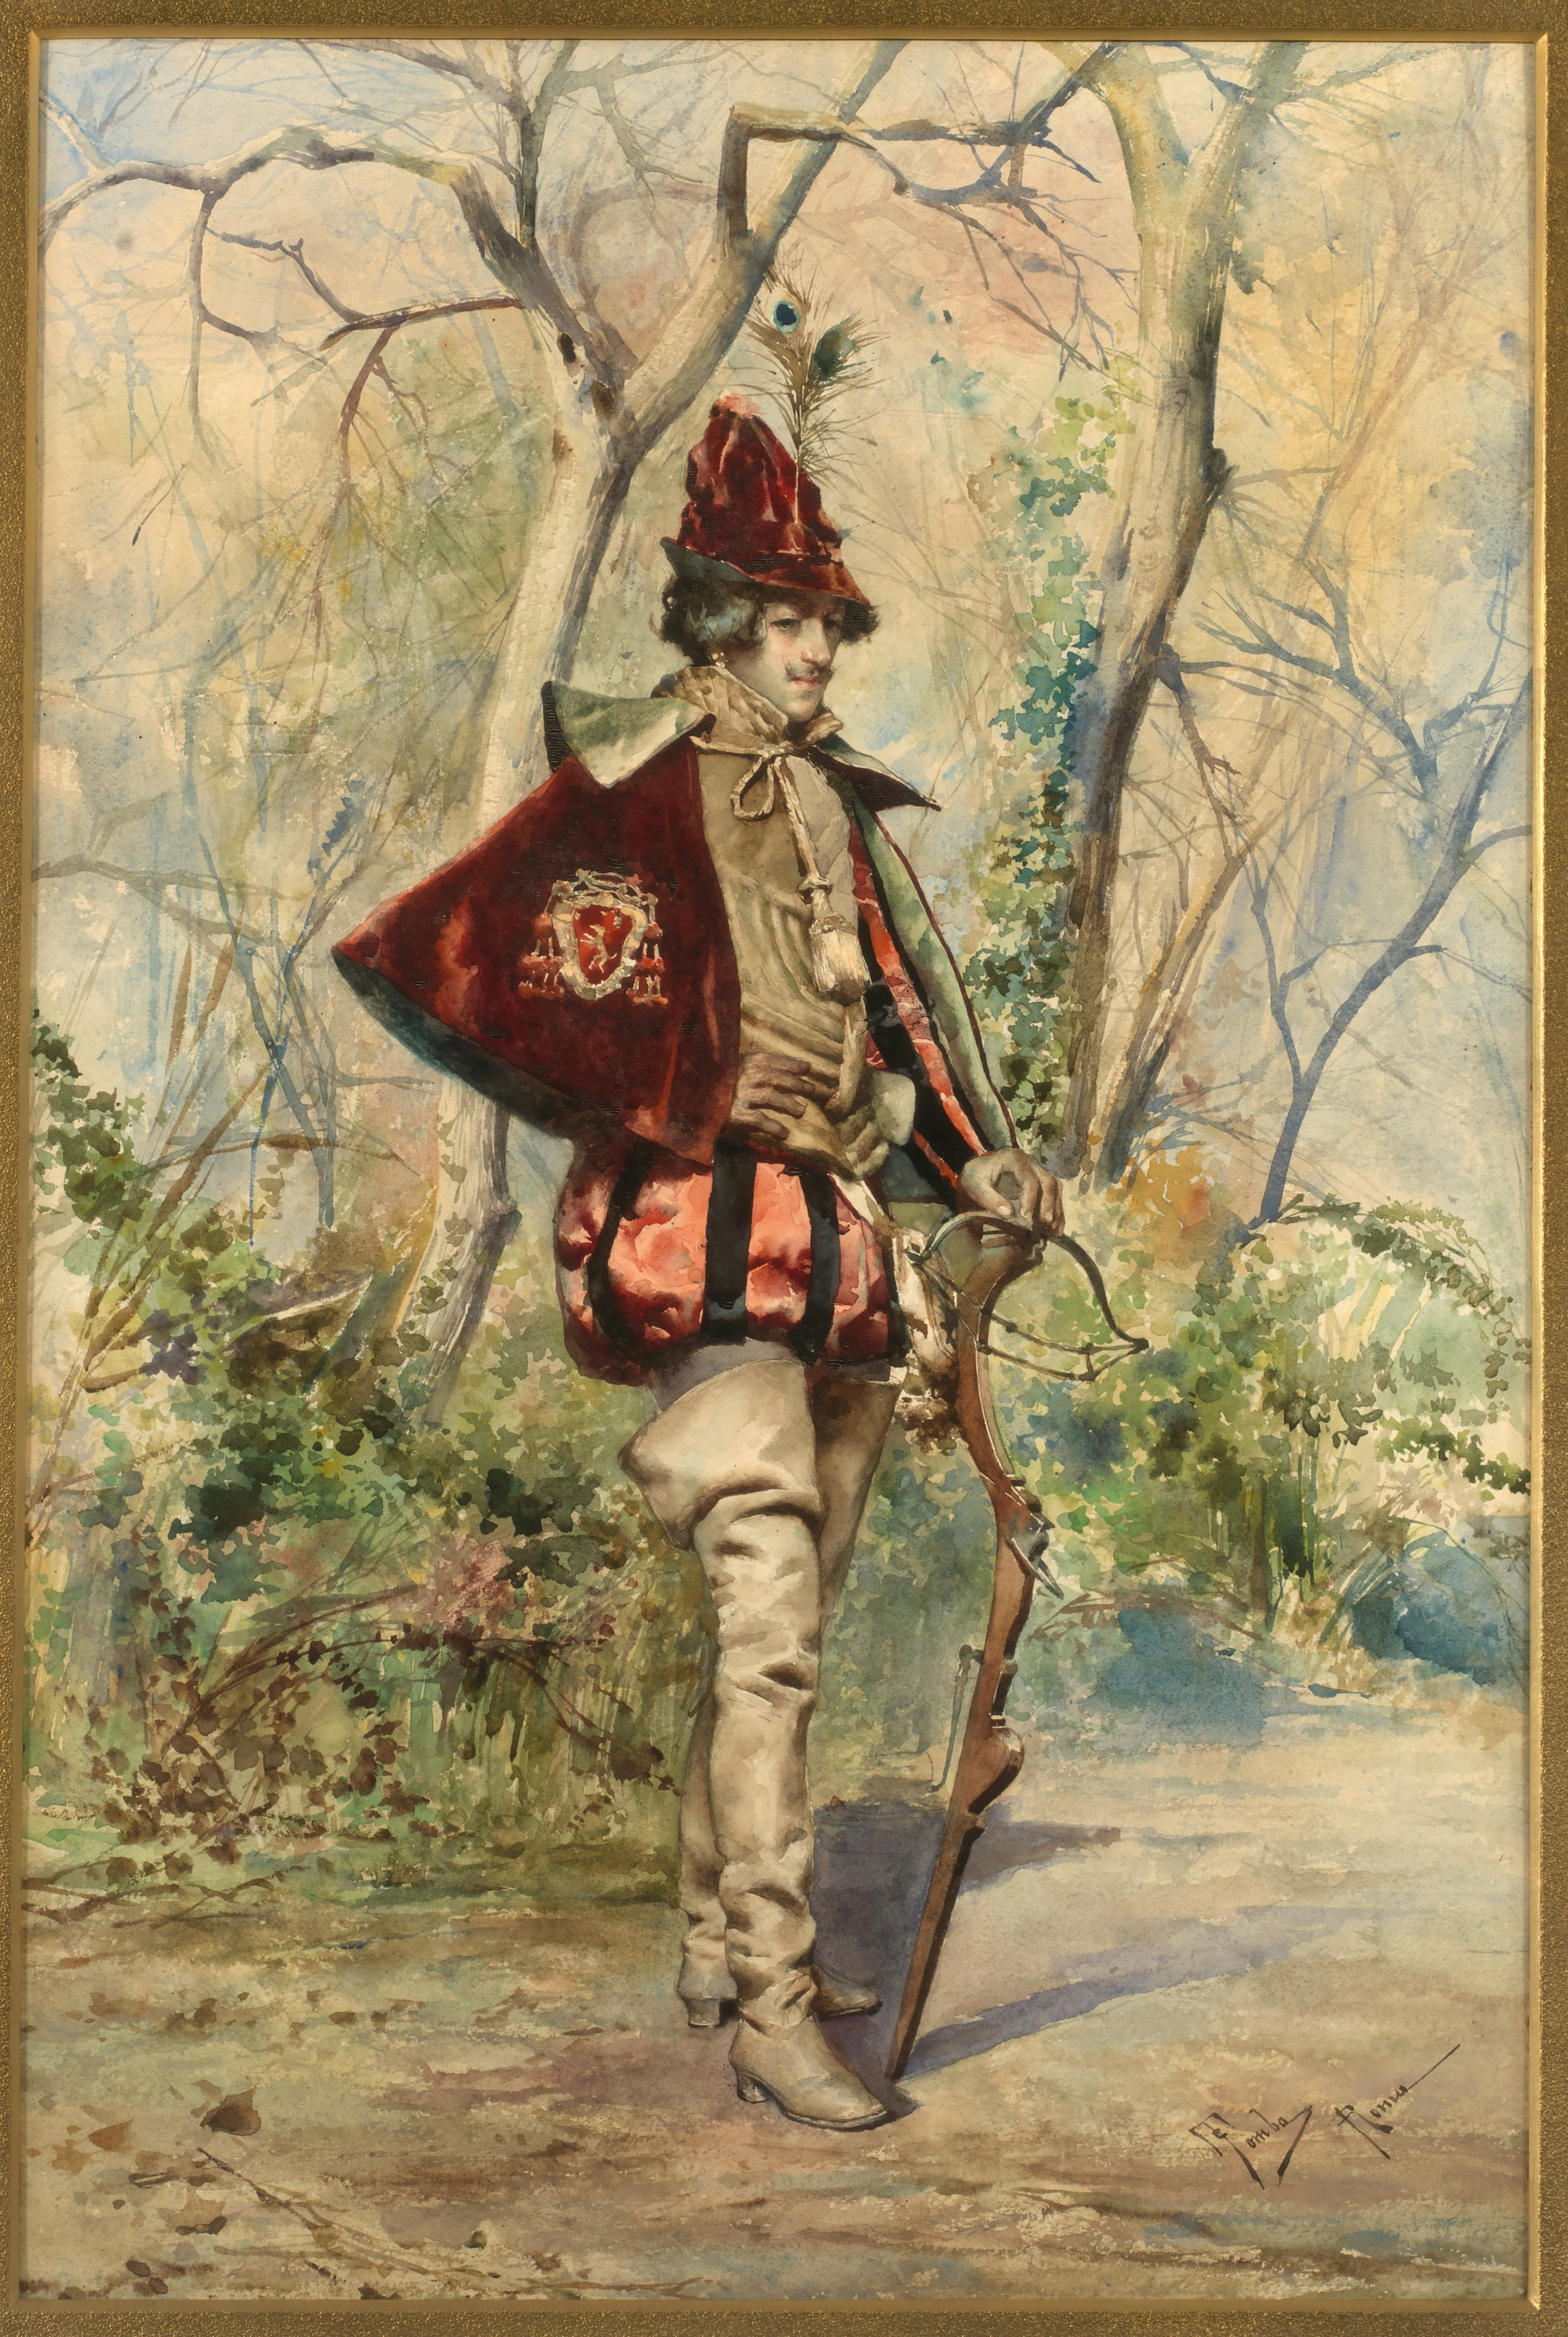
\includegraphics[width=\paperwidth,height=\paperheight]{cover.jpg}
    };
\definecolor{shadecolor}{gray}{0.9}
\vfill
\begin{shaded}
    \begin{center}
        \HUGE\textsf{\thetitle}
    \end{center}

    \begin{center}
        \LARGE\textsf{\theauthor}
    \end{center}
\end{shaded}

\cleardoublepage

% half-title page
\begin{center}
\HUGE\textsf{\thetitle}
\end{center}
\cleardoublepage

% title page
\begin{center}
\HUGE\textsf{\thetitle}
\end{center}

\begin{center}
\LARGE\textsf{\theauthor}
\end{center}
\clearpage

% copyright page
\begingroup
\footnotesize
\setlength{\parindent}{0pt}
\setlength{\parskip}{\baselineskip}

\textcopyright{} 2024 Destination Infinity / Rajesh Kollu

All rights reserved. No part of this book can be copied or reproduced anywhere
without the written consent of the author. This is a work of fiction. All events
in this story are purely imaginary and resemblance to anyone dead/alive is sheer
coincidence.

\endgroup
\clearpage

\begin{quote}
\begin{center}Dedicated to

\LARGE
Mrs. P. Vijayalakshmi
\normalsize

My Tamil Language Teacher @ D.A.V, Chennai
\end{center}
\end{quote}

\vfill

\textbf{Acknowledgements}
% typeset this with tables

Romila (Proof Reader/Editor) – onlymeinc@yahoo.com


Abhishek Singh (Marketing Support) – http://kebooks.com

My Mother (Beta Reader).


\clearpage